% !TeX spellcheck = de_DE
\section{Algoritmer til detektering af gang, løb og cykling}
\textit{Dette afsnit omhandler design, implementering og test af algoritmerne til detektering af gang, løb og cykling. Først designes algoritmerne til det specifikke formål, hvorefter de kan implementeres. Afslutningsvist bliver algoritmerne testet i forhold til opstillede krav i \secref{krav_algoritme}.} 
%bliver design af algoritmerne behandlet, hvilket er ensbetydende med at implementering og kodning kan foregå. Når algoritmerne er designet og implementeret bliver de efterfølgende testet for at af- eller bekræfte deres virkning.}

\subsection{Design}
For at kunne adskille gang, løb og cykling benyttes et accelerometer og et gyroskop, som er beskrevet i \secref{sec_design_LSM9DS1}. Gyroskopet skal benyttes til at detektere cykling, mens løb og gang detekteres ved brug af accelerometeret. For at kunne detektere og adskille disse aktiviteter behandles inputtet fra sensorerne gennem forskellig signalbehandlingsprocessor. Algoritmerne gør det muligt at afgøre, om de pågældende signaler repræsenterer gang, løb, cykling eller ingen fysisk aktivitet. 

\subsubsection{Algoritme til detektion af gang og løb} \label{design_algo_g_l}
Data fra accelerometerets y-akse skal signalbehandles, førend en algoritme kan detektere samt adskille gang og løb. Første trin i denne signalbehandling er at fjerne støj ved brug af et elliptisk filter. Dette skal være et fjerde ordens elliptisk båndpasfilter med et pasbånd fra 20 til 50 Hz, og med en dæmpning på 60 dB\fxnote{og 0.5 dB peak-to-peak ripples - frekvenserne for gang og løb lå mellem 25 og 45}. Båndpasfilterets knækfrekvenser er bestemt gennem pilotforsøget i \appref{pilot}, hvorudfra det vurderes at hælnedslag findes ved cirka 25 Hz og signalet herfra stopper omkring 45 Hz. Alt inden for disse frekvenser burde derfor indeholde det vigtigste i signalet.\fxnote{Der er også meget lavfrekvent støj med meget høj amplitude, men det er vi ikke interesseret i, fordi det er f.eks. svingfasen.} Dermed frafiltreres eventuel 50 Hz støj fra signalet samt lavfrekvent DC signal. %. Knækfrekvensen omkring 20 Hz er bestemt for at bibeholde signalets hælnedslag, hvoraf frekvensen befandt sig omkring 20 Hz. 
Andet trin i signalbehandlingen består af, at det filtrede signal divideres med 36. Dette gøres ved hjælp af en implementeret funktion i PSoC. Signalets amplituder bliver heraf formindsket, og de mindste amplituder nærmer sig nul i større grad end amplituden for hælnedslag. Derved gøres peaket for dette tydligere. I det tredje trin i signalbehandlingen bliver signalet kvadreret ved hjælp af en funktion i PSoC programmer. Dette medfører, at de dele af signalet med lav amplitude under 1 formindskes, mens andre dele af signalet med amplituder over værdien 1 forstærkes. Dermed minimeres de events kraftigt, som ikke relateres til hælnedslaget, og selve hælnedslaget forstærkes.\fxnote{ved gang er det swing og heel strike, ved løb er det primært kun heel strike, men også lidt toe offset.} Fjerde og sidste trin i signalbehandlingen bliver signalet filtreret med et moving average filter, som udglatter signalet, hvorved små udslag ikke opfattes, og signalets hælnedslag vil fremstå som et enkelt event.

Ovenstående signalbehandling giver et endeligt signal med peaks, som skal adskilles med tærskelværdier for henholdsvis gang og løb. Førend en værdi for denne tærskelværdi kan fastsættes, skal dataet fra pilotforsøgets omregnes til ICens arbejdsområde. ICens arbejdsområde er opgivet i bytes af dets 16 bits ADC arbejdsområde. Konverteringen til denne enhed skal gøres ved Shimmer, da enheden er $m/s^{2}$. Først skal dataet omregnes fra denne enhed til g, hvilket gøres ved at dividere med tyngdekræften. Efterfulgt af dette skal enheden omregnes til Shimmers arbejdsområde vedrørende dets 12 bit ADC arbejdsområde. For at gøre dette benyttes accelerometerets sensitivitet, som er 0,012 g/LSB. Data fra shimmer som er omregnet til g, skal divideres med accelerometerets sensitivitet. Outputet fra Shimmer og ICen er nu samme enhed, men ikke samme størrelse. Dette er et resultat af at de ikke besidder samme ADC.
 
\begin{equation}
\frac{32 g \times 2^{16}}{32 g \times 2^{12}} = 16
\label{eq:bitsammenhaeng}
\end{equation}

Data fra Shimmer skal ganges med 16 for at være sammen størrelsesorden, hvilket er et resultat af at Shimmer benytter 12 bit ADC, og ICen besidder en 16 bit ADC. Ud fra konvertering af data samt algoritmens signalbehandling, vurderes det, at amplituden for hælnedslag ved løb overskrider en outputværdi på 400 og ved gang overskrider en outputværdi på 50 for alle forsøgspersoner. Derfor vil events med amplituder under 50 vurderes som værende inaktivitet.
\begin{figure}[H]
	\centering
	\includegraphics[scale=0.5]{figures/cDesign/algoritme_gl.png}
	\caption{På figuren ses et flowchart over algoritmen til detektering af gang og løb.}
	\label{fig:algoritme}
\end{figure}
Ovenstående \figref{fig:algoritme} repræsenterer algoritmen for detektering og adskillelsen af gang og løb. Førend algoritmen tilhørende gang og løb starter, undersøges det hvorvidt cykling registreres. Hvis dette er tilfældet, påbegyndes algoritmen for cykling, som ses på \textbf{HENVIS TIL PSEUDO FIGUREN FOR CYKLING!}. Hvis cykling ikke registreres, vil data fra accelerometret blive signalbehandlet. \\
En timer skal aktiveres, når algoritmen registrerer ingen aktivitet, gang eller løb, der adskilles ved hjælp af to tærskelværdier. Timeren nulstilles hver gang et maks peak går under en defineret tærskelværdi. Hvis dette maks peak ligger inden for samme tærskelværdi som forrige maks peak, skal timerens tid summeres med den forrige, således der kommer en samlet tid for den pågældende aktivitet. Dette kommer dog til at finde sted i algoritmen for GUIen. Når timeren nulstiller, sendes tidsenheden herfra altså videre samt værdien for den registrerede maks peak. Værdien herfra definerer netop, om der er tale om ingen aktivitet, gang eller løb. Timeren skal stoppe helt, hvis cykling registreres i stedet, da der findes en separat timer i algoritmen til detektion af cykling. %Herefter startes timeren igen opg. Hvis løb ikke detekteres, undersøges der hvorvidt gang registreres. Hvis gang registreres skal en timer ligeledes først stoppe når gang ikke længere detekteres. Når timeren stopper sendes varigheden som en tidsværdi for udført gang og max peak registeres og sendes ligeledes. Herefter startes timeren igen. 
Hvis algoritmen til detektering af gang og løb ikke registrer aktiviteterne, bliver der ikke udført nogen bevægelse eller cykling finder sted, hvorfor algoritmen starter forfra indtil detektering af gang eller løb. \\
Fælles for både detektering af gang og løb er, at første målte peak samt det første peak efter tre sekunder uden aktivitet kasseres. Dette gøres for at sikre en periode uden aktivitet ikke summeres som faktisk gang eller løb.

\subsubsection{Algoritme til detektion af cykling}\label{design_cykling}
Data fra gyroskopets z-akse skal signalbehandles, førend en algoritme kan detektere cykling og adskille denne fra gang og løb. Første trin i denne signalbehandling er at udføre en Fast Fourier Transform (FFT) over fire sekunders sampling. Dette medfører, at signalets frekvenser og deres tilhørende magnituder kommer til udtryk. I andet trin findes frekvensværdien for den maksimale peak. Amplituden herfra bliver summeret i det tredje trin sammen med amplituderne for $\pm$1 Hz af den pågældende frekvens med maks peak. Derved fås en amplitudeværdi for maks peak værdien summeret med de to omkringliggende amplitudeværdier. Derudover summeres amplitudeværdierne for FFTen fra 1 til 20 Hz i det tredje trin, som herefter vil blive betegnet som hele FFTen. Resultatet heraf består i en amplitudeværdi for den maksimale peak med omkringliggende værdier, samt en amplitude værdi for hele FFTen. Resultaterne af disse to summeringer benyttes til fjerde og sidste trin, som omregner hvor stor en procentdel den første summering med det højeste peak udgør i forhold til den samlede FFT. Summeringen over den maksimale peak med omkringliggende værdier vil typisk udgøre en stor procentdel af den samlede summering. Resultatet af at summeringen udgør en stor procentdel af den samlede energi, er at cykling afspejles som et sinussignal, hvoraf energien befinder sig omkring få frekvenser. Aktiviteterne gang og løb har ikke samme karakteristiske påvirkning af gyroskopet.
\begin{figure}[H]
	\centering
	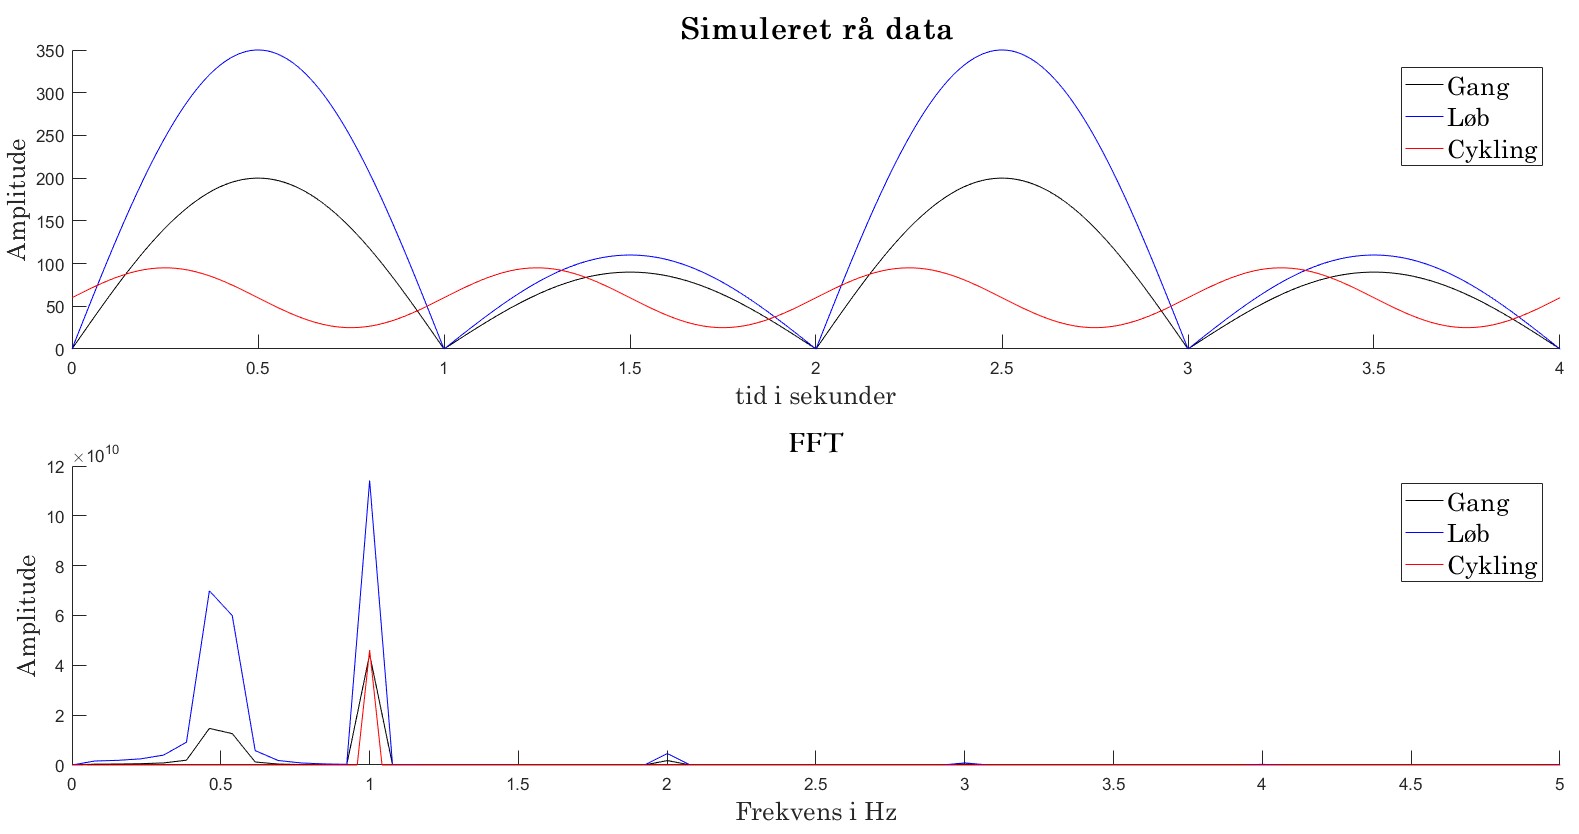
\includegraphics[scale=0.8]{figures/cDesign/gyro_behandling.png}
	\caption{Figuren viser rå data for gang, løb og cykling for et 5 sekunders interval opsamlet på gyroskopets z-akse på øverste graf, samt signalbehandling af dataet fra 0 til 20~Hz på nederste graf.}
	\label{fig:gyro_behandling}
\end{figure}\vspace{-0.5cm}
Data fra pilotforsøget er behandlet med ovenstående signalbehandling. Dette er gjort med henblik på fastsættelse af en tærskelværdi som adskiller cykling fra gang og løb. På den øverste graf på \figref{fig:gyro_behandling} ses de rå signaler fra gyroskopet fra gang, løb og cykling. Som det tydelig ses afspejles cykling tilnærmelsesvis som en sinus, hvorfor dennes energi er centreret omkring få frekvenser. Resultatet af den omtalte signalbehandling ses på den nederste graf, hvoraf gang, løb og cykling er blevet behandlet med en FFT. Hertil ses det også at energien for gang og løb ikke centrerer sig omkring en enkelt frekvens, men om forskellige frekvenser, hvoraf denne spredning af energi kan benyttes til signalgenkendelse og adskillelse af aktiviteterne. 

Efter ovenstående signalbehandlingen implementeres signalgenkendelsen som består af, først at finde den maksimale magnitude og den tilhørende frekvens, resultatet heraf er aktivitetens dominerende frekvens. Herefter summeres værdierne for den maksimale magnitude, ved at summere intervallet $\pm$1~Hz omkring frekvens heraf. Hertil summeres også værdierne for FFTen fra 1 til 20~Hz. Afslutningsvist bestemmes hvor stor en procentdel summeringen for den maksimale magnitude udgør af summeringen for 1 til 20~Hz.\\ 

\begin{table}[H]
	\centering
	\resizebox{\textwidth}{!}{%
	\begin{tabular}{cccc}
		\hline
		\rowcolor[HTML]{C0C0C0} 
		Forsøgsperson & Procentdel af totalen for gang & Procentdel af totalen for løb & Procentdel af totalen for cykling \\ \hline
		F1 & 41,0\% & 38,6\% & 85,5\% \\ \hline	
		F2 & 48,5\% & 51,5\% & 91,9\% \\ \hline	
		F3 & 35,9\% & 42,8\% & 85,0\% \\ \hline
		F4 & 38,7\% & 60,6\% & 91,6\% \\ \hline
	\end{tabular}
}
	\caption{I tabellen ses hvor stor en procentdel summeringen vedrørende den maksimale magnitude udgør af hele FFTen. Dette er gjort for både gang, løb og cykling, med henblik på bestemmelse af en tærskelværdi.}
	\label{tab:individuel_procent}
\end{table}\vspace{-0.5cm}
Mængden af energi ved den maksimale magnitude er markant større for cykling i forhold til gang og løb, hvilket er illustreret i \tabref{tab:individuel_procent}. Dette resulterede i, at 84,5\% til 91,9\% af energien lå $\pm$1 Hz omkring den fundne frekvens med den største amplitude. Hvorledes acceleration eller andre hastigheder ved cykling har påvirkning på denne procentfordeling diskuteres i \secref{sec:diskussion}. Procentfordelingen blev ligeledes behandlet for gang og løb for at sikre, at disse ikke havde samme spredning i frekvensområdet, hvormed en mulig tærskelværdi til detektering af cykling kan fastsættes. Resultatet heraf medførte at ved gang befandt energien omkring den fundne frekvens sig mellem 35,9\% til 48,5\% og ved løb befandt energien omkring den fundne frekvens sig mellem 42,8\% til 60,5\%. Denne forskel benyttes til at adskille cykling fra gang og løb, ved at implementere et tærskelværdi på 70\%. Summeringen af magnituden omrking den største magnitude skal dermed udgøre 70\% for at blive klassificeret som cykling. 
\begin{figure}[H]
	\centering
	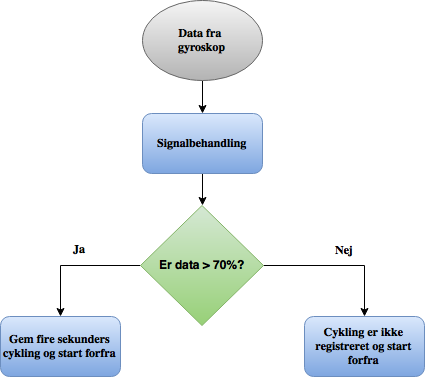
\includegraphics[scale=0.6]{figures/cDesign/algoritme_cykling.png}
	\caption{På figuren ses et flowchart som gennemgår algoritmen vedrørende detektering af cykling.}
	\label{fig:algoritme_cykling}
\end{figure}
Ovenstående figur repræsenterer algoritmen for detektering af cykling. Hvis cykling detekteres, starter en time count, som stopper når cykling ikke længere detekteres. Når timeren stopper, videresendes timerens værdi som repræsenterer tiden hvormed cykling har været detekteret. Hvis cykling ikke detekteres, signalbehandles ny data fra gyroskopet, for at tjekke hvorvidt cykling detekteres.  

\subsection{Implementering}
\subsubsection{Algoritme til detektion af gang og løb}
Implementeringen af algoritmen for detektering af gang og løb tager udgangspunkt i data fra pilotforsøg og består grundlæggende af to delelementer. Først signalbehandling hvorefter selve algoritmen implementeres. Signalbehandlingen er blevet implementeret som egenfunktioner i C, hvoraf signalet bliver behandlet med fire funktioner, førend data bliver kørt igennem algoritmen. De fire funktioner er som sagt et elliptisk filter, division med 32, kvadrering og mooving average filter. \\
For at finde filterkoefficienterne til det elliptiske filter anvendes MATLAB. Herinde skrives knækfrekvenserne samt dæmpningsgraden for et elliptisk filter, hvorefter programmet giver a og b koefficienterne. Disse skrives ind i PSoC programmer som et IIR filter som double float type. Denne funktion kan initialisere større tal og er mere præcis i forhold til kommatal. Efter filtreringen divideres og kvadreres dataet, som til sidst behandles af et mooving average filter i PSoC creater, hvorfor behandlingen vil ske på MCUen.

Betydningen af databehandlingen for signalet kan ses på \figref{fig:algoritme_cykling2}
\begin{figure}[H]
	\centering
	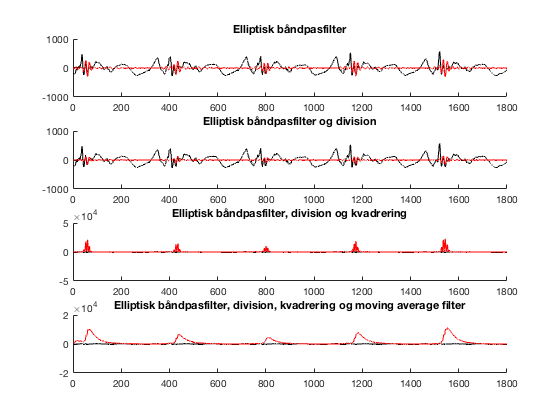
\includegraphics[width=1\textwidth]{figures/cDesign/signalbehandling_psoc.png}
	\caption{På figuren ses de fire signalbehandlingsfunktioners effekt på rå accelerometer data fra løb. Den sorte kurve på de fire figurer er det rå signal, og den røde er det behandlede output. Der gøres opmærksom på, at y-aksen ikke er ens for henholdsvis de to øvre og de to nedre figurer, hvorfor det sorte, rå signal bliver en næsten lige linje på de to nedre figurer.}
	\label{fig:algoritme_cykling2}
\end{figure}
Funktionaliteten af ovenstående signalbehandling sikre, at signalet for hælnedslagets bliver så markant, således tærskelværdier til detektering og adskillelse af gang og løb er mulig. Det behandlede output antages som værende repræsentativt for, hvordan PSoC vil behandle realtids data, når det endelige system er færdigt. Dette antages, da det er data fra pilotforsøget i \appref{pilot}, som er blevet behandlet igennem PSoC og derefter visualiseret. Data fra pilotforsøget er for alle forsøgspersoner blevet behandlet med ovenstående signalbehandling med henblik på fastsættelse af tærskelværdier. 
\begin{table}[H]
	\centering
	\begin{tabular}{ccc}
		\hline
		\rowcolor[HTML]{C0C0C0} 
		Forsøgsperson & Tærskelværdi for gang & Tærskelværdi for løb \\ \hline
		\rowcolor[HTML]{FFFFFF} 
		F1 & 50 & 1050 \\ \hline
		\rowcolor[HTML]{FFFFFF} 
		F2 & 55 & 500 \\ \hline
		\rowcolor[HTML]{FFFFFF} 
		F3 & 50 & 400 \\ \hline
		\rowcolor[HTML]{FFFFFF} 
		F4 & 150 & 100 \\ \hline
	\end{tabular}
	\caption{I tabellen ses tærskelværdierne for forsøgspersonerne vedrørende aktiviteterne gang og løb.}
	\label{tab:individuel_taerskel}
\end{table}\vspace{-0.5cm}
De individuelle tærskelværdier i \tabref{tab:individuel_taerskel} er fundet over et fem sekunders vindue for hver forsøgsperson. Heraf antages det, at tærskelværdierne bør være dækkende for hele målingen, da forsøgspersonerne udførte aktiviteterne ved konstant hastighed. I vinduet for hver forsøgspersons data bliver det vurderet, hvor en tærskelværdi vil være bedst placeret, således maks peak detekteres. En samlet tærskelværdi, der er dækkende for samtlige forsøgspersoners data, ses i \tabref{tab:faelles_taerskel}.
\begin{table}[H]
	\centering
	\begin{tabular}{ccc}
		\hline
		\rowcolor[HTML]{C0C0C0} 
		Tærskelværdi for ingen aktivitet & Tærskelværdi for gang & Tærskelværdi for løb \\ \hline
		x \textless 50 & x \textgreater 50 \& x \textless 400 & x =\textgreater 400 \\ \hline
	\end{tabular}
	\caption{I tabellen ses de tærskelværdier, som for alle forsøgspersoner vil kunne detektere og adskille gang og løb fra hinanden.}
	\label{tab:faelles_taerskel}
\end{table}\vspace{-0.5cm}
Fastsættelsen af den fælles tærskelværdi bør sikre, at gang og løb er mulige at detektere samt adskille for forsøgspersonernes data. Igennem behandling af data fra pilotforsøget forekom tærskelværdierne i \tabref{tab:faelles_taerskel} dækkende for alle forsøgspersonerne, hvorfor disse blev valgt.

Tærskelværdierne implementeres i PSoC creater i if lykker. Her hentes data fra databehandlingen ind, hvorefter if lykkerne skal afgøre, om dataet er under laveste, mellem eller over højeste tærskelværdi. Hvis data er under laveste tærskelværdi, bliver timeren ikke udløst til at nulstille sig men fortsætter med at tælle i tre sekunder, hvorefter den nulstilles og tæller igen til tre. Det første detekterede maks peak efter ingen aktivitet registreres ikke, da timeren skal tælle fra forrige tilfælde af, at signalet går under tærskelværdien og til den næste. Det første maks peak efter en periode uden aktivitet vil derfor have en ukorrekt time counter værdi, da det kan være fra nul til tre sekunder lang. \\% har ikke noget forrige maks peak at sammenholde med, hvorved time counteren vil give ukorrekt output.
Ved hjælp af if lykkerne behandles det databehandlede signal som henholdsvis ingen aktivitet, gang og løb, hvorigennem specifikt data sendes videre. Data sendes videre ved brug af UART forbindelsen, som kaldes i PSoC Creater.

\subsubsection{Algoritme til detektion af cykling}
Implementeringen af algoritmen for detektering af cykling tager udgangspunkt i data fra pilotforsøget og de designmæssige aspekter, som er beskrevet i \secref{design_cykling}. Algoritmen er designet og implementeret, som det ses på \figref{fig:basic_cykling}.
\begin{figure}[H]
	\centering
	\includegraphics[scale=0.4]{figures/cDesign/Algoritme_cykling_basic.png}
	\caption{På figuren ses den kode for algoritmen til detektering cykling beskrevet med pesudokode. Den røde markerede kasse vil blive forklaret yderligere en kommende figur.}
	\label{fig:basic_cykling}
\end{figure}
Algoritmen henter low-, og high byte fra ICens gyroskop outputdata, hvorefter hver enkelt sample videresendes til MATLAB, som gemmer 4 sekunders data i et arrary og påbegynder signalbehandlingen. Resultatet af signalbehandlingen medfører en procentvis værdi for det modtagne data. Denne værdi undersøges for at være over eller under tærskelværdien. Hvis resultatet er over 70\% summeres fire sekunder til den totale varighed for cykling, hvis ikke startes algoritmen forfra.
\begin{figure}[H]
	\centering
	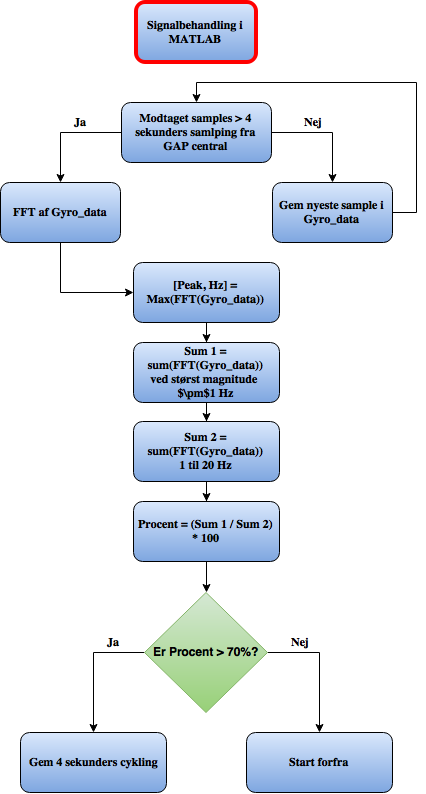
\includegraphics[scale=0.4]{figures/cDesign/algoritme_matlab_cykling.png}
	\caption{På figuren ses den kode for algoritmens signalbehandling i MATLAB.}
	\label{fig:matlab_cykling}
\end{figure} 
Når MATLAB har modtaget fire sekunders sampling påbegyndes signalbehandlingen af dataet ved brug at formlerne i \figref{fig:matlab_cykling}. Hvis cykling bliver detekteret bliver en varighed på fire sekunder videresendt til udført cykling i GUI. 



\subsection{Test}
\subsubsection{Algoritme til detektion af gang og løb}
Algoritmens funktioner testes individuelt og samlet. Dette gøres ved at indsende et simuleret signal, hvis funktion er at agerer som gang, løb eller ingen aktivitet. Det simulerede signal er et absolut sinussignal med varierende amplitude. Amplituden for det simulerede signal afgør, hvorvidt signalet bør agerer som gang, løb eller ingen aktivitet. Et sinussignal er valgt, da dette har grundlæggende samme karateristik som et eventuelt gang- eller løbesignal. Der ønskes et ideelt signal, som går over og under tærskelværdierne og derved kan aktivere timeren i algoritmen.

Først testes algoritmens time counter, der giver et udtryk for, om algoritmen detekterer gang korrekt. Der indsendes et absolut sinussignal samplet med 512 Hz, en frekvens på 0,5 Hz og en amplitude på 100. Dette resulterede i tre halvbølger med en amplitude på 100 på 1536 samples. Dette kan ses som den sorte kurve på \figref{fig:testgraf_timecounter}.
\begin{figure}[H]
	\centering
	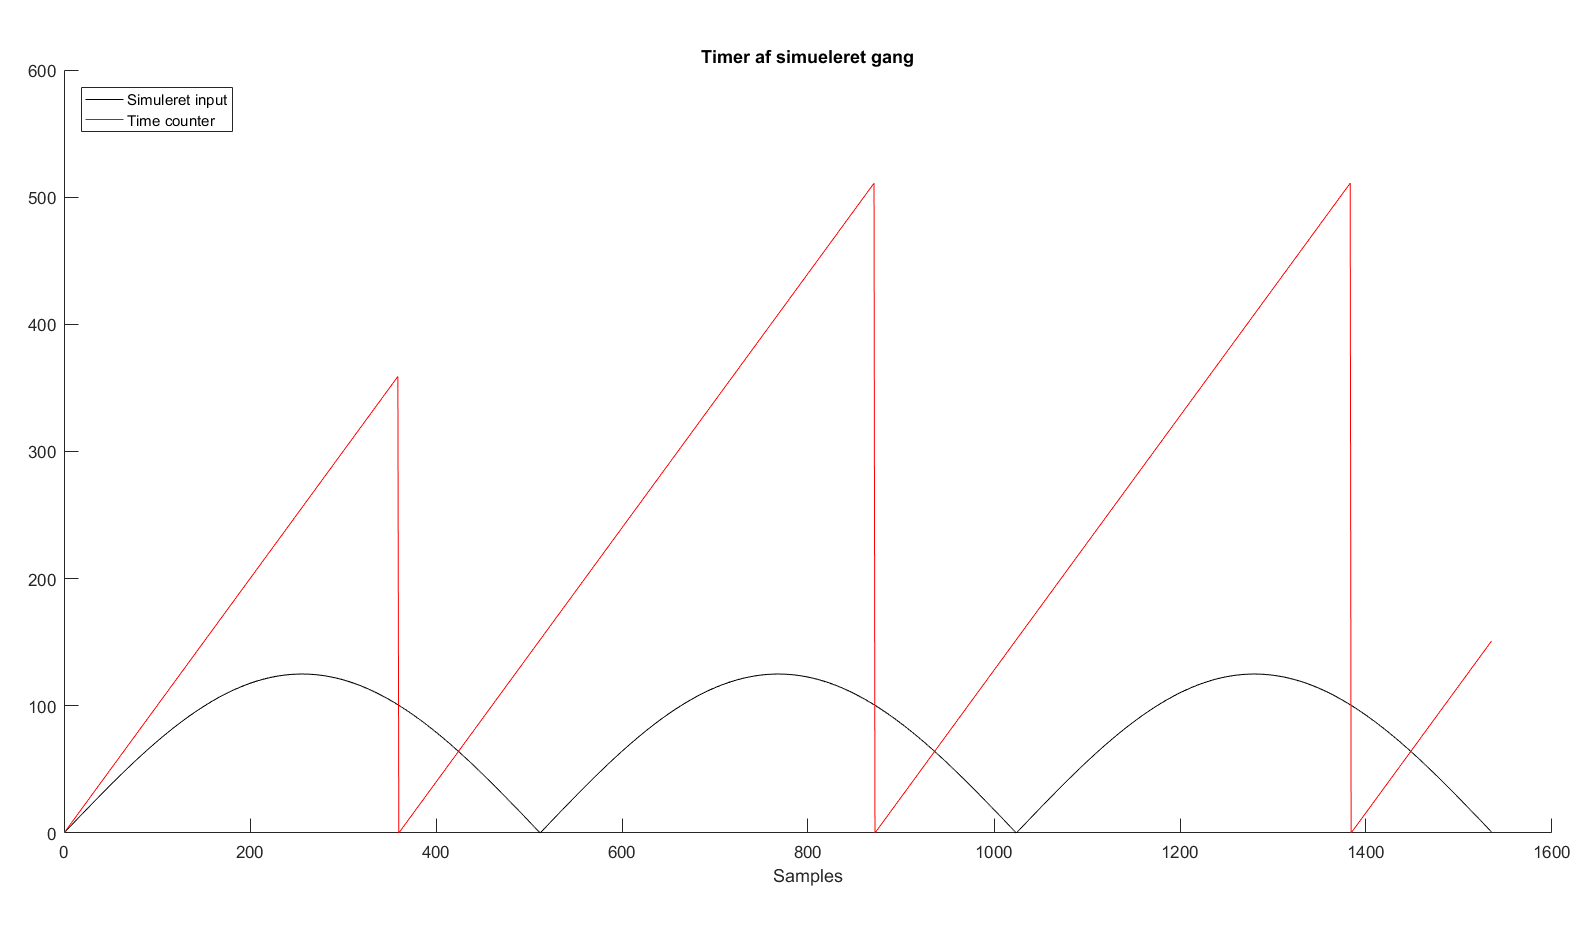
\includegraphics[width=.9\textwidth]{figures/cDesign/test_timecount_gang.png}
	\caption{På figuren ses algoritmens time counter som den røde kurve, der reagerer på detekteringen af et simuleret gangsignal. Denne nulstilles hver gang signalet går under tærskelværdien, således maks peak værdien og tidsværdien sendes videre. Den sorte kurve er det simulerede gangsignal.}
	\label{fig:testgraf_timecounter}
\end{figure}
Algoritmens time counter starter, når signalet bliver indsendt, og nulstilles efter en sample går under tærskelværdien. Heraf kan det ses, at varigheden fra en sample er gået under en tærskelværdi til, at en sample igen er gået under en tærskelværdi er 512 samples. En af algoritmens funktioner er at frasortere det første detekterede peak, dermed nulstille time counter værdien samt peak værdien.\\
Den egentlige test vedrørende algoritmens time counter består dermed i at undersøge, om den første peak tælles med eller ej i videresendt data. I \tabref{tab:test_res_timecount} ses der, at selvom den første peak visualiseres i \figref{fig:testgraf_timecounter}, så medregnet den ikke i de endelige værdier. Disse værdier fås ved hjælp af programmet Realterm, som viser sendt data fra MCUen ved brug af UART.
\begin{table}[H]
	\centering
	\begin{tabular}{ccc}
		\hline
		\rowcolor[HTML]{C0C0C0} 
		Værdi videresendt & Forventet værdi [samples] & Modtaget værdi [samples] \\ \hline
		Time counter & $\emptyset$ - 512 - 512 & $\emptyset$ - 512 - 512 \\ \hline
	\end{tabular}
	\caption{I tabellen ses testresultaterne vedrørende test af time counter. $\emptyset$ antyder at det ikke blev modtaget noget ved første peak.}
	\label{tab:test_res_timecount}
\end{table} \vspace{-0.5cm}
Algoritmen er blevet testet på tre halvbølger, og dermed er det forventede resultat at varigheden af første peak ikke blev medregnet og videresendt som et resultat. Algoritmens time counter fungerede som forventet, og videresendte kun det forventede resultat med præcis nøjagtighed. Denne del af algoritmen accepteres og er klar til implementering i det samlede system.

I anden test af algoritmen tjekkes der for, om algoritmen giver korrekt værdi for maks peak detektering. Denne er designet således, at algoritmen ikke skal registrer det første peak i et signal, som første test beviste ikke sker. På \figref{fig:test_peak_gang} ses resultatet af testen.
\begin{figure}[H]
	\centering
	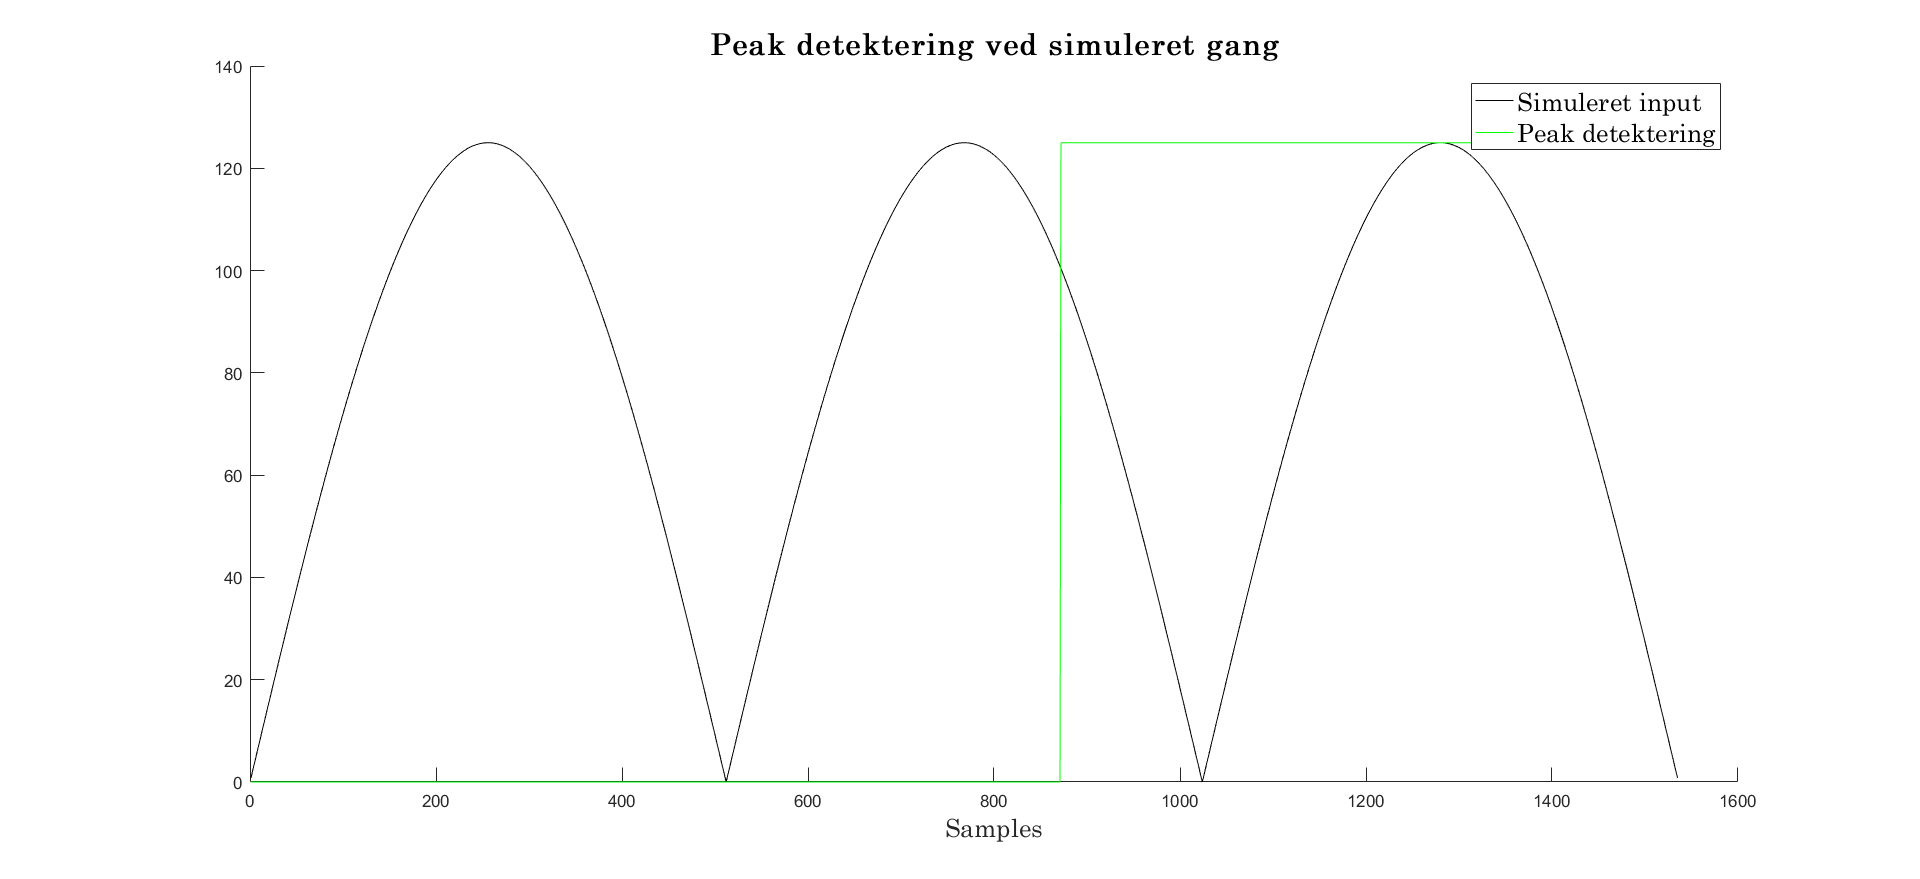
\includegraphics[width=.9\textwidth]{figures/cDesign/test_peak_gang.png}
	\caption{På figuren ses algoritmens funktion til at detektere værdien for maks peak i et simuleres gangsignal. Den sorte kurve er det simulerede gang signal, og den røde kurve viser algoritmens funktion til detektering af peakværdier. Der ses, at den første peak ikke detekteres som ønsket. Herefter findes værdien for det andet maks peak, når signalet er gået under tærskelværdien på 50. Da tredje maks peak har samme værdi som anden maks peak, forbliver den røde kurve på samme værdi.}
	\label{fig:test_peak_gang}
\end{figure}\vspace{-.5cm}
Algoritmens detektering af peak starter, når en sample overskrider en bestemt tærskelværdi, hvilket ikke fremgår tydeligt på \figref{fig:test_peak_gang}. Men algoritmen finder maks peaket, når en sample er under tærskelværdien, hvilket ses ud fra den røde graf. Hvis det første peak detekteres, sættes værdien til nul, således den ikke tælles med. På \figref{fig:test_peak_gang} kan det ses, at når signalet går under tærskelværdien anden gang, bliver peaket registreret. Den egentlige test vedrørende algoritmens detektering af peaks består dermed i at undersøge hvilke data, der videresendes som resultat, efter et input er kørt igennem algoritmen. Resultatet heraf ses i \tabref{tab:test_res_peak}, som fås ved hjælp af programmet Realterm, som viser sendt data fra MCUen ved brug af UART.
\begin{table}[H]
	\centering
	\begin{tabular}{ccc}
		\hline
		\rowcolor[HTML]{C0C0C0} 
		Værdi videresendt & Forventet output [amplitude] & Output [amplitude] \\ \hline
		Peak detektering & $\emptyset$ - 100 - 100 & $\emptyset$ - 100 - 100 \\ \hline
	\end{tabular}
	\caption{I tabellen ses testresultaterne vedrørende test af detektering af peaks. $\emptyset$ antyder at det ikke blev modtaget noget ved første peak. Der ses i tabellen, at outputtet fra testen stemmer overens med det forventede output.}
	\label{tab:test_res_peak}
\end{table}\vspace{-0.5cm}
Algoritmen er blevet testet på tre halvbølger, og dermed er det forventede resultat, at peakværdien af det første peak ikke bliver medregnet og videresendt som et resultat. Algoritmens peak detektering fungerer dermed som forventet og videresendte amplituderne, som halvbølgerne var designet med, med en præcis nøjagtighed. Denne del af algoritmen accepteres og er klar til implementering i det samlede system.

Algoritmen for løb blev ligeledes testet med hensyn til funktionaliteten af time counter og peak detektering. Ved denne test blev der indsendt et absolut sinussignal med en højere amplitude, som ville overskride tærskelværdien vedrørende detektering af løb. Resultaterne af disse test medførte resultater af samme nøjagtighed, som ved detektering af gang. Algoritmen bør dermed fungerer optimalt, både til detektering af gang og løb men testet herunder i samlet plots.

Algoritmen bør altså undersøge, hvorvidt data fra accelerometret klarificeres som ingen aktivitet, gang eller løb ved hjælp af tærskelværdier. I testen heraf indsendes et simuleret signal, som først overskrider tærskelværdierne for gang på 50. Herefter forekommer en periode på tre sekunder, hvor hverken gang eller løbs tærskelværdi overskrides, hvorfor time counteren vil nulstille efter tre sekunder uden overskridelse af nogen tærskelværdier. Afslutningsvis indsendes værdier, som overskrider tærskelværdierne vedrørende løb på 400. Herigennem bliver både time count og detektering af peaks testet, hvilket fremgår i \figref{fig:test_inaktiv_time} og \figref{fig:test_inaktiv_peak}. 
\begin{figure}[H]
	\centering
	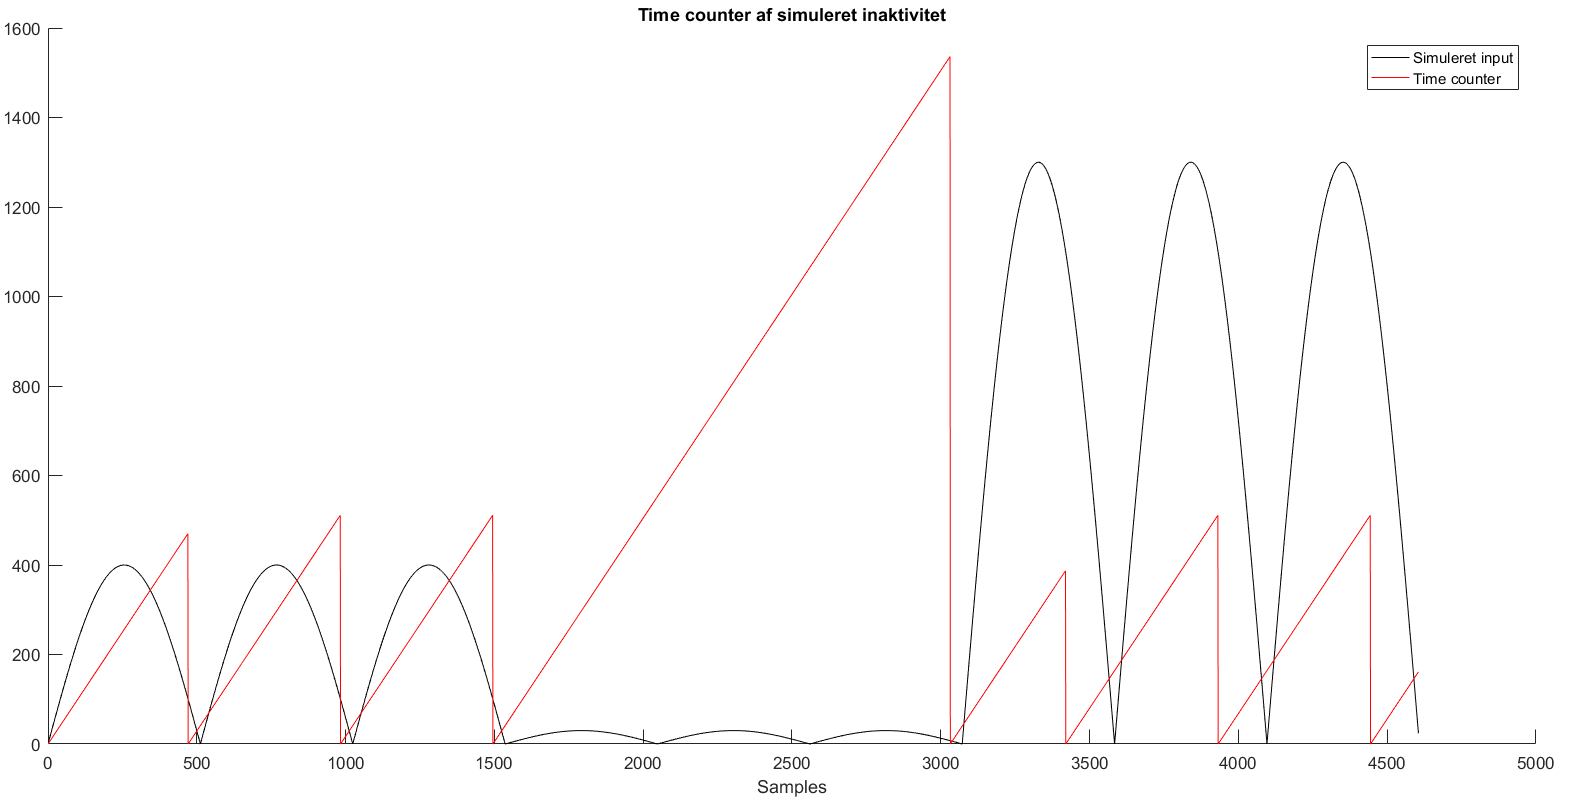
\includegraphics[scale=0.3]{figures/cDesign/test_timecount_inaktiv.png}
	\caption{På figuren ses algoritmens time counter, som resultat af detektering af et simuleret gang, inaktiv og løbe signal. Den sorte kurve er det simulerede signal, og den røde kurve viser algoritmens time counter af samples, som overholder algoritmens specifikationer. Der ses i midten af figuren, at time counteren nulstilles efter tre sekunder selvom inden tærskelværdier er overskredet. Det er derfor fordelagtigt at smide værdien ud for første detekterede maks peak herefter.}
	\label{fig:test_inaktiv_time}
\end{figure}

\begin{figure}[H]
	\centering
	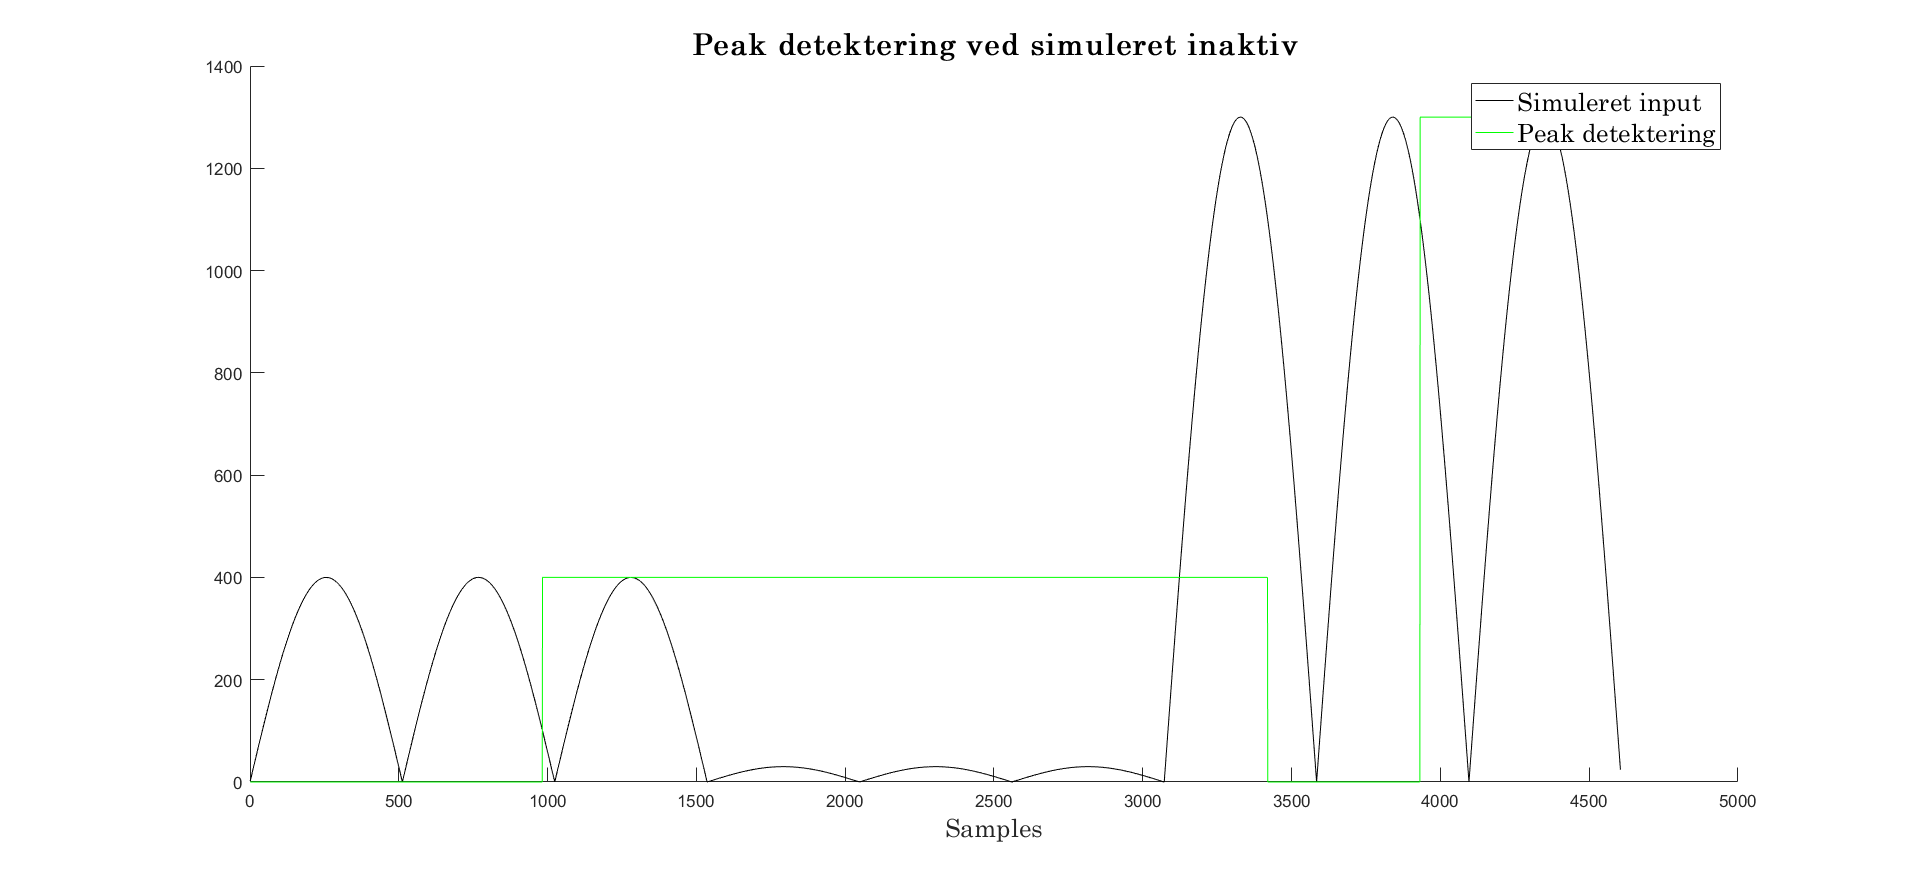
\includegraphics[width=.9\textwidth]{figures/cDesign/test_peak_inaktiv.png}
	\caption{På figuren ses algoritmens funktion til at detektere peakværdier, som resultat af detektering af et simuleret gang, inaktiv og løbe signal. Den sorte kurve er det simulerede signal, og den røde kurve er algoritmens funktion til detektering af peakværdier. }
	\label{fig:test_inaktiv_peak}
\end{figure}
Resultaterne vedrørende time count på \figref{fig:test_inaktiv_time} viser, at i perioden uden nogen aktivitet nulstilles time counteren ikke, før en sample har været over og under en tærskelværdi. Resultaterne vedrørende detektering af peak på \figref{fig:test_inaktiv_peak} viser, at første værdi tilhørende det første peak, samt det første peak efterfulgt fra ingen aktivitet frasorteres. For at klassificere hvorvidt algoritmen omhandlende detektering af ingen aktivitet fungerer efter hensigten, undersøges det data, der bliver videresendt som et resultat af perioder uden aktivitet. I tilfælde med et signalinput som ovenstående bør det første peak frasorteres efterfulgt af to værdier. Resultatet fra denne test fremgår i \tabref{tab:test_inaktiv}. %Derudover bør der registreres to time count værdier med tilhørende peakværdier efterfulgt af en periode med inaktivitet, hvoraf første peak frasorteres og dermed to time count værdier med tilhørende peak værdier.
\begin{table}[H]
	\centering
	\begin{tabular}{ccc}
		\hline
		\rowcolor[HTML]{C0C0C0} 
		Værdi videresendt & Forventet værdi & Modtaget værdi \\ \hline
		Time counter [samples] & $\emptyset$ - 512 - 512 - $\emptyset$ - 512 - 512 & $\emptyset$ - 512 - 512 - $\emptyset$ - 512 - 512 \\ \hline
		\multicolumn{1}{l}{Peak detektering [amplitude]} &     \multicolumn{1}{l}{$\emptyset$ - 200 - 200 - $\emptyset$ - 600 - 600}     &     \multicolumn{1}{l}{$\emptyset$ - 200 - 200 - $\emptyset$ - 600 - 600} \\ \hline
	\end{tabular}
	\caption{I tabellen ses testresultaterne vedrørende test af time count og detektering af peak ved et simuleret signal, som illustrerer en periode uden aktivitet. $\emptyset$ antyder at det ikke blev modtaget noget ved første peak. Der ses i tabellen, at algoritmen agerer efter hensigten.}
	\label{tab:test_inaktiv}
\end{table}\vspace{-0.5cm}
Algoritmen er blevet testet på et simuleret signal, som skulle illustrer en periode uden aktivitet omringet af to perioder med henholdsvis gang og løb. Det forventede resultat for både time count værdien og peakværdien er, at det første peak frasorteres, og første peak efter en periode uden aktivitet frasorteres. Dermed forventes det, at det videresendte data er time count på 512, og amplituder som afspejler signalets design på 200 og 600. Resultatet af det data, som blev modtaget, var som forventet med præcis nøjagtighed, og dermed kan det antages at algoritmens funktion vedrørende detektering af perioder uden aktivitet fungerer efter hensigten. Denne del af algoritmen accepteres og er klar til implementering i det samlede system.

\subsubsection{Algoritme til detektion af cykling}
\textit{Er ikke lavet endnu.}

